%%%%%%%%%%%%%%%%%%%%%%%%%%%%%%%%%%%%%%%%%%%%%%%%%%%%%%%%%%%%%%%%%%%%%%%%%%%%%%%%%%%%%%%%%%%%%%%%%%%%%%%%%%%%%%%%%%%%%%%%%%%%%%%%%%%%%%%%%%%%%%%%%%%%%%%%%%%
% This is just an example/guide for you to refer to when submitting manuscripts to Frontiers, it is not mandatory to use Frontiers .cls files nor frontiers.tex  %
% This will only generate the Manuscript, the final article will be typeset by Frontiers after acceptance.
%                                              %
%                                                                                                                                                         %
% When submitting your files, remember to upload this *tex file, the pdf generated with it, the *bib file (if bibliography is not within the *tex) and all the figures.
%%%%%%%%%%%%%%%%%%%%%%%%%%%%%%%%%%%%%%%%%%%%%%%%%%%%%%%%%%%%%%%%%%%%%%%%%%%%%%%%%%%%%%%%%%%%%%%%%%%%%%%%%%%%%%%%%%%%%%%%%%%%%%%%%%%%%%%%%%%%%%%%%%%%%%%%%%%

%%% Version 3.3 Generated 2016/11/10 %%%
%%% You will need to have the following packages installed: datetime, fmtcount, etoolbox, fcprefix, which are normally inlcuded in WinEdt. %%%
%%% In http://www.ctan.org/ you can find the packages and how to install them, if necessary. %%%
%%%  NB logo1.jpg is required in the path in order to correctly compile front page header %%%

\documentclass[utf8]{frontiersSCNS} % for Science, Engineering and Humanities and Social Sciences articles
%\documentclass[utf8]{frontiersHLTH} % for Health articles
%\documentclass[utf8]{frontiersFPHY} % for Physics and Applied Mathematics and Statistics articles

%\setcitestyle{square} % for Physics and Applied Mathematics and Statistics articles
\usepackage{url,hyperref,lineno,microtype,subcaption}
\usepackage[onehalfspacing]{setspace}

\linenumbers


% Leave a blank line between paragraphs instead of using \\


\def\keyFont{\fontsize{8}{11}\helveticabold }
\def\firstAuthorLast{Sample {et~al.}} %use et al only if is more than 1 author
\def\Authors{Brian A. Cohn\,$^{1,*}$, Kian Jalaleddini\,$^{2}$ and Francisco J. Valero-Cuevas\,$^{1,2}$}
% Affiliations should be keyed to the author's name with superscript numbers and be listed as follows: Laboratory, Institute, Department, Organization, City, State abbreviation (USA, Canada, Australia), and Country (without detailed address information such as city zip codes or street names).
% If one of the authors has a change of address, list the new address below the correspondence details using a superscript symbol and use the same symbol to indicate the author in the author list.
\def\Address{$^{1}$Laboratory X, Institute X, Department X, Organization X, City X , State XX (only USA, Canada and Australia), Country X \\
$^{2}$Laboratory X, Institute X, Department X, Organization X, City X , State XX (only USA, Canada and Australia), Country X  }
% The Corresponding Author should be marked with an asterisk
% Provide the exact contact address (this time including street name and city zip code) and email of the corresponding author
\def\corrAuthor{Francisco J. Valero-Cuevas}

\def\corrEmail{valero@usc.edu}


\begin{document}
\onecolumn
\firstpage{1}

\title[Motor learnability across posture]{Motor learnability across posture}

\author[\firstAuthorLast ]{\Authors} %This field will be automatically populated
\address{} %This field will be automatically populated
\correspondance{} %This field will be automatically populated
\extraAuth{}% If there are more than 1 corresponding author, comment this line and uncomment the next one.
%\extraAuth{corresponding Author2 \\ Laboratory X2, Institute X2, Department X2, Organization X2, Street X2, City X2 , State XX2 (only USA, Canada and Australia), Zip Code2, X2 Country X2, email2@uni2.edu}


\maketitle

\keyFont{ Abstract: Z Words, Body: X Words, Pages: Y}
\\
\begin{abstract}

Learning algorithms applied to tendon-driven limbs are not rigorously tested on robotic or cadaveric tissues in a way that systematically permutes posture and noise.
Furthermore, the amount of data required to measure the mechanical component of neuromotor noise is unclear.
There exists a gap between the mechanical properties of cadaveric tendon-driven limbs across realistic positions, and the models that describe how tendon forces affect the limb's endpoint force behavior.
We addressed this limitation by inventing a tension-to-force experiment that collects data across hundreds of isometric endpoint postures of any tendon-driven limb controlled by up to 10 newtons per tendon.
We experimented with a bioinspired robotic finger as a stand-in for a cadaveric finger, attached a six-dimensional force sensor at its fingertip, we wound tension-controlled strings about its joints in an arbitrary routing.
The fingertip fit snugly in the force sensor, which was affixed to a manipulator---that way, we were able to move the posture with sub millimeter precision, in under 2 seconds.
Using the resultant data (with 1000 postures along a line and 100 tensions across 7-tendons for each posture) we (i) characterized static and dynamic components of the tension-to-force relationship, (ii) identified specific postures that are more challenging to control accurately, (iii) compared the performance of models from the literature (linear, dynamic, and linear-cascade), (iv) and evaluated the robustness of results under differing sample size and noise.
Our contribution empowers artificial intelligence experts to develop robust interpretations of a model's performance atop data from a postural workspace, thereby enabling biologically-inspired tactile sensing from the muscle properties themselves.
In capturing the variables associated with posture-specific tendon-driven control, we open a new front for thorough understanding of the biomechanical constraints and pressures across in learning, health, disease, and in an evolutionary context.

\tiny
 \keyFont{ \section{Keywords:} motor control, force control, neuroscience, tendon-driven systems, isometric, force production, posture} %All article types: you may provide up to 8 keywords; at least 5 are mandatory.
\end{abstract}

\section{Introduction}

"cable driven flexion and extension" apparatus was built of flexible material, and, importantly, was not aligned with joints specifically \cite{Yi:2018et}. This highlights how our understanding of squishy tendon-driven limbs must take into account that nervous systems are happy to work with squishiness. Our robotic approach to neuroscience limits us.

\section{Results}
Further analyses:

%TODO kian see if there is a good figure/analysis to explore this:
What is the relationship between posture, and the amount of force variability after settling?


\subsection{Heading Levels}

%There are 5 heading levels

\subsection{Level 2}
\subsubsection{Level 3}
\paragraph{Level 4}
\subparagraph{Level 5}


\section{Discussion}
\subsection{Noise in signal}

%TODO Kian
where does the noise come from?
how would we reduce that?
is it important that we reduce that? how does variability/noise in our muscle forces over time compare to noise in a normal EMG, or normal isometric tendon task.

\section*{Conflict of Interest Statement}
The authors declare that the research was conducted in the absence of any commercial or financial relationships that could be construed as a potential conflict of interest.

\section*{Author Contributions}
BC and KJ designed the experiment.
BAC designed and programmed analytics and served as the lead scientist.
KJ implemented the motor control modules, calibrated sensor equipment, and provided insight into the dynamical response of the limb.
FV provided a thoughtful angle to the implications of this research on the fields of neuroscience, artificial intelligence, and robotics.

\section*{Funding}
Research was supported by the National Institute of Arthritis and Musculoskeletal and Skin Diseases of
the National Institutes of Health (NIH) under Awards Number R01 AR-050520 and R01 AR-052345 to FVC, and
the National Science Foundation Graduate Research Fellowship Program Award to BAC.
The content is solely the responsibility of the authors and does not necessarily represent the official views of the NIH or NSF.

\section*{Acknowledgments}
We thank <KIAN TODO Add Posture Dependency Interns>, M Ishikawa, T Stroobosscher, and B Miura for their instrumental support in mechanical and electrical engineering, as well as support with analytics reviews and documentation.

\bibliographystyle{frontiersinSCNS_ENG_HUMS} % for Science, Engineering and Humanities and Social Sciences articles, for Humanities and Social Sciences articles please include page numbers in the in-text citations
\bibliography{test}

\begin{figure}[h!]
\begin{center}
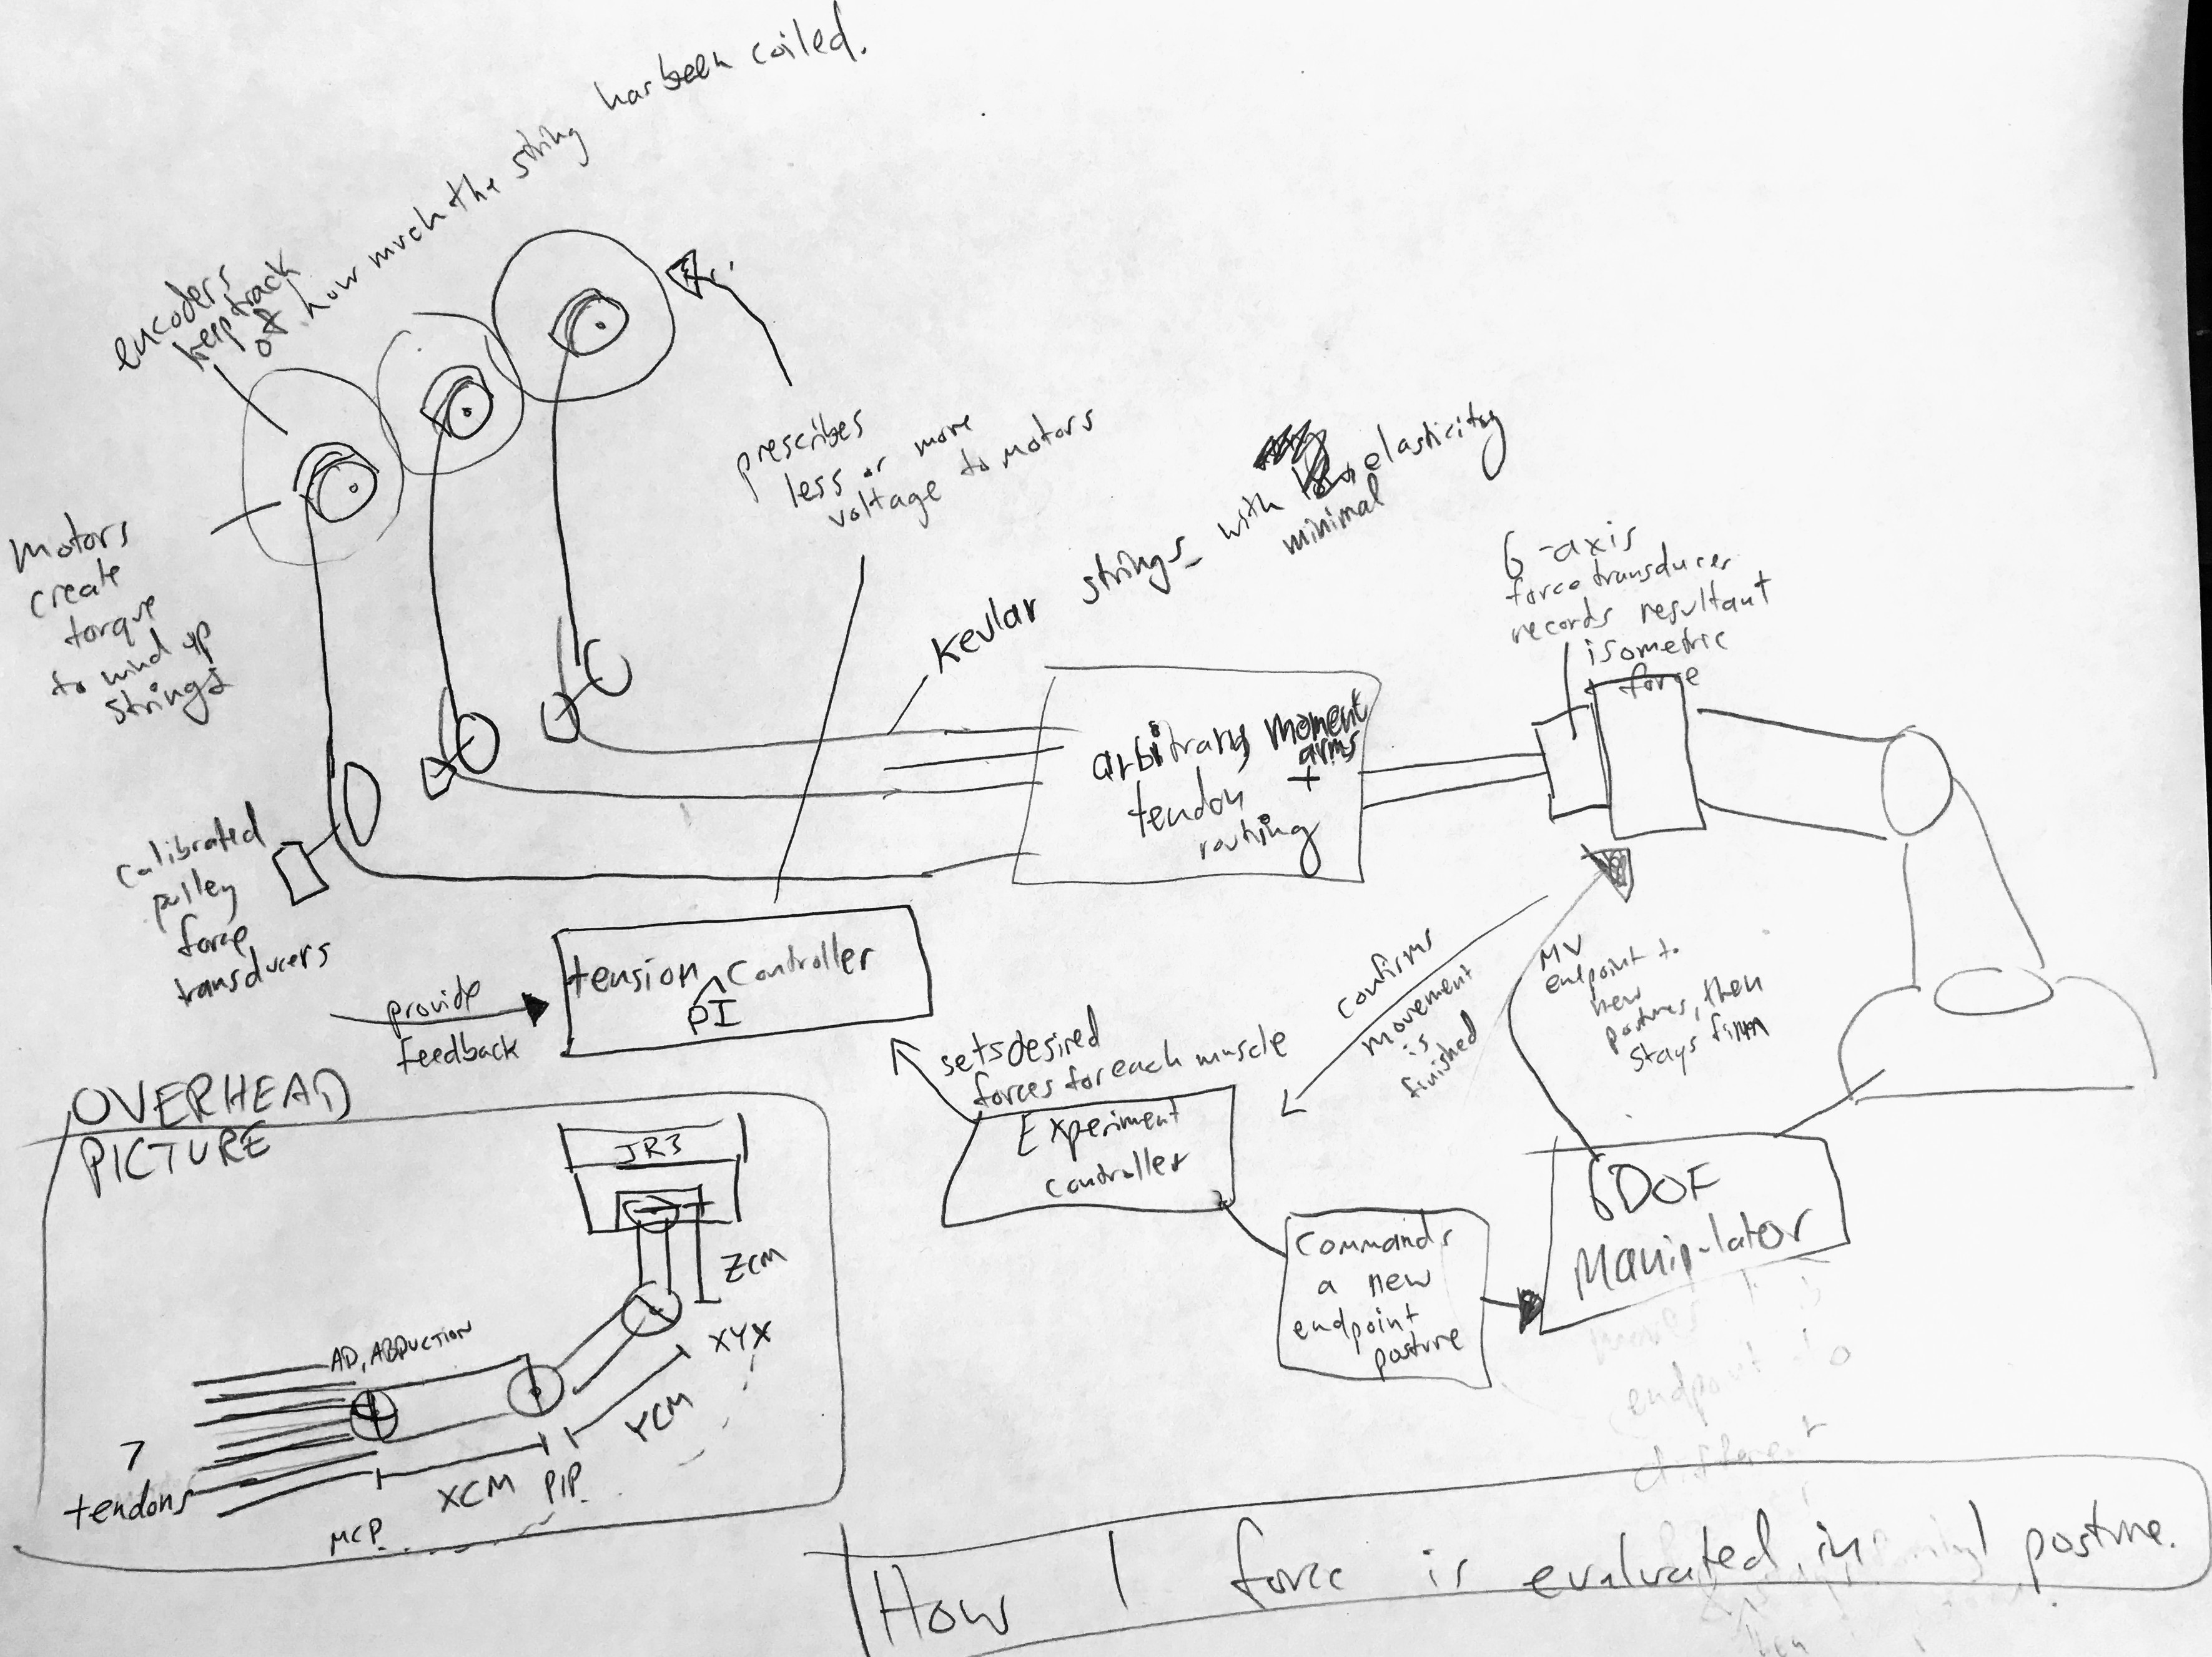
\includegraphics[width=17.5cm]{figures/overview/overview.jpg}% This is a *.jpg file
\end{center}
\caption{Experimental paradigm for all posture dependency experiments.}
\label{fig:overview}
\end{figure}

\begin{figure}[h!]
\begin{center}
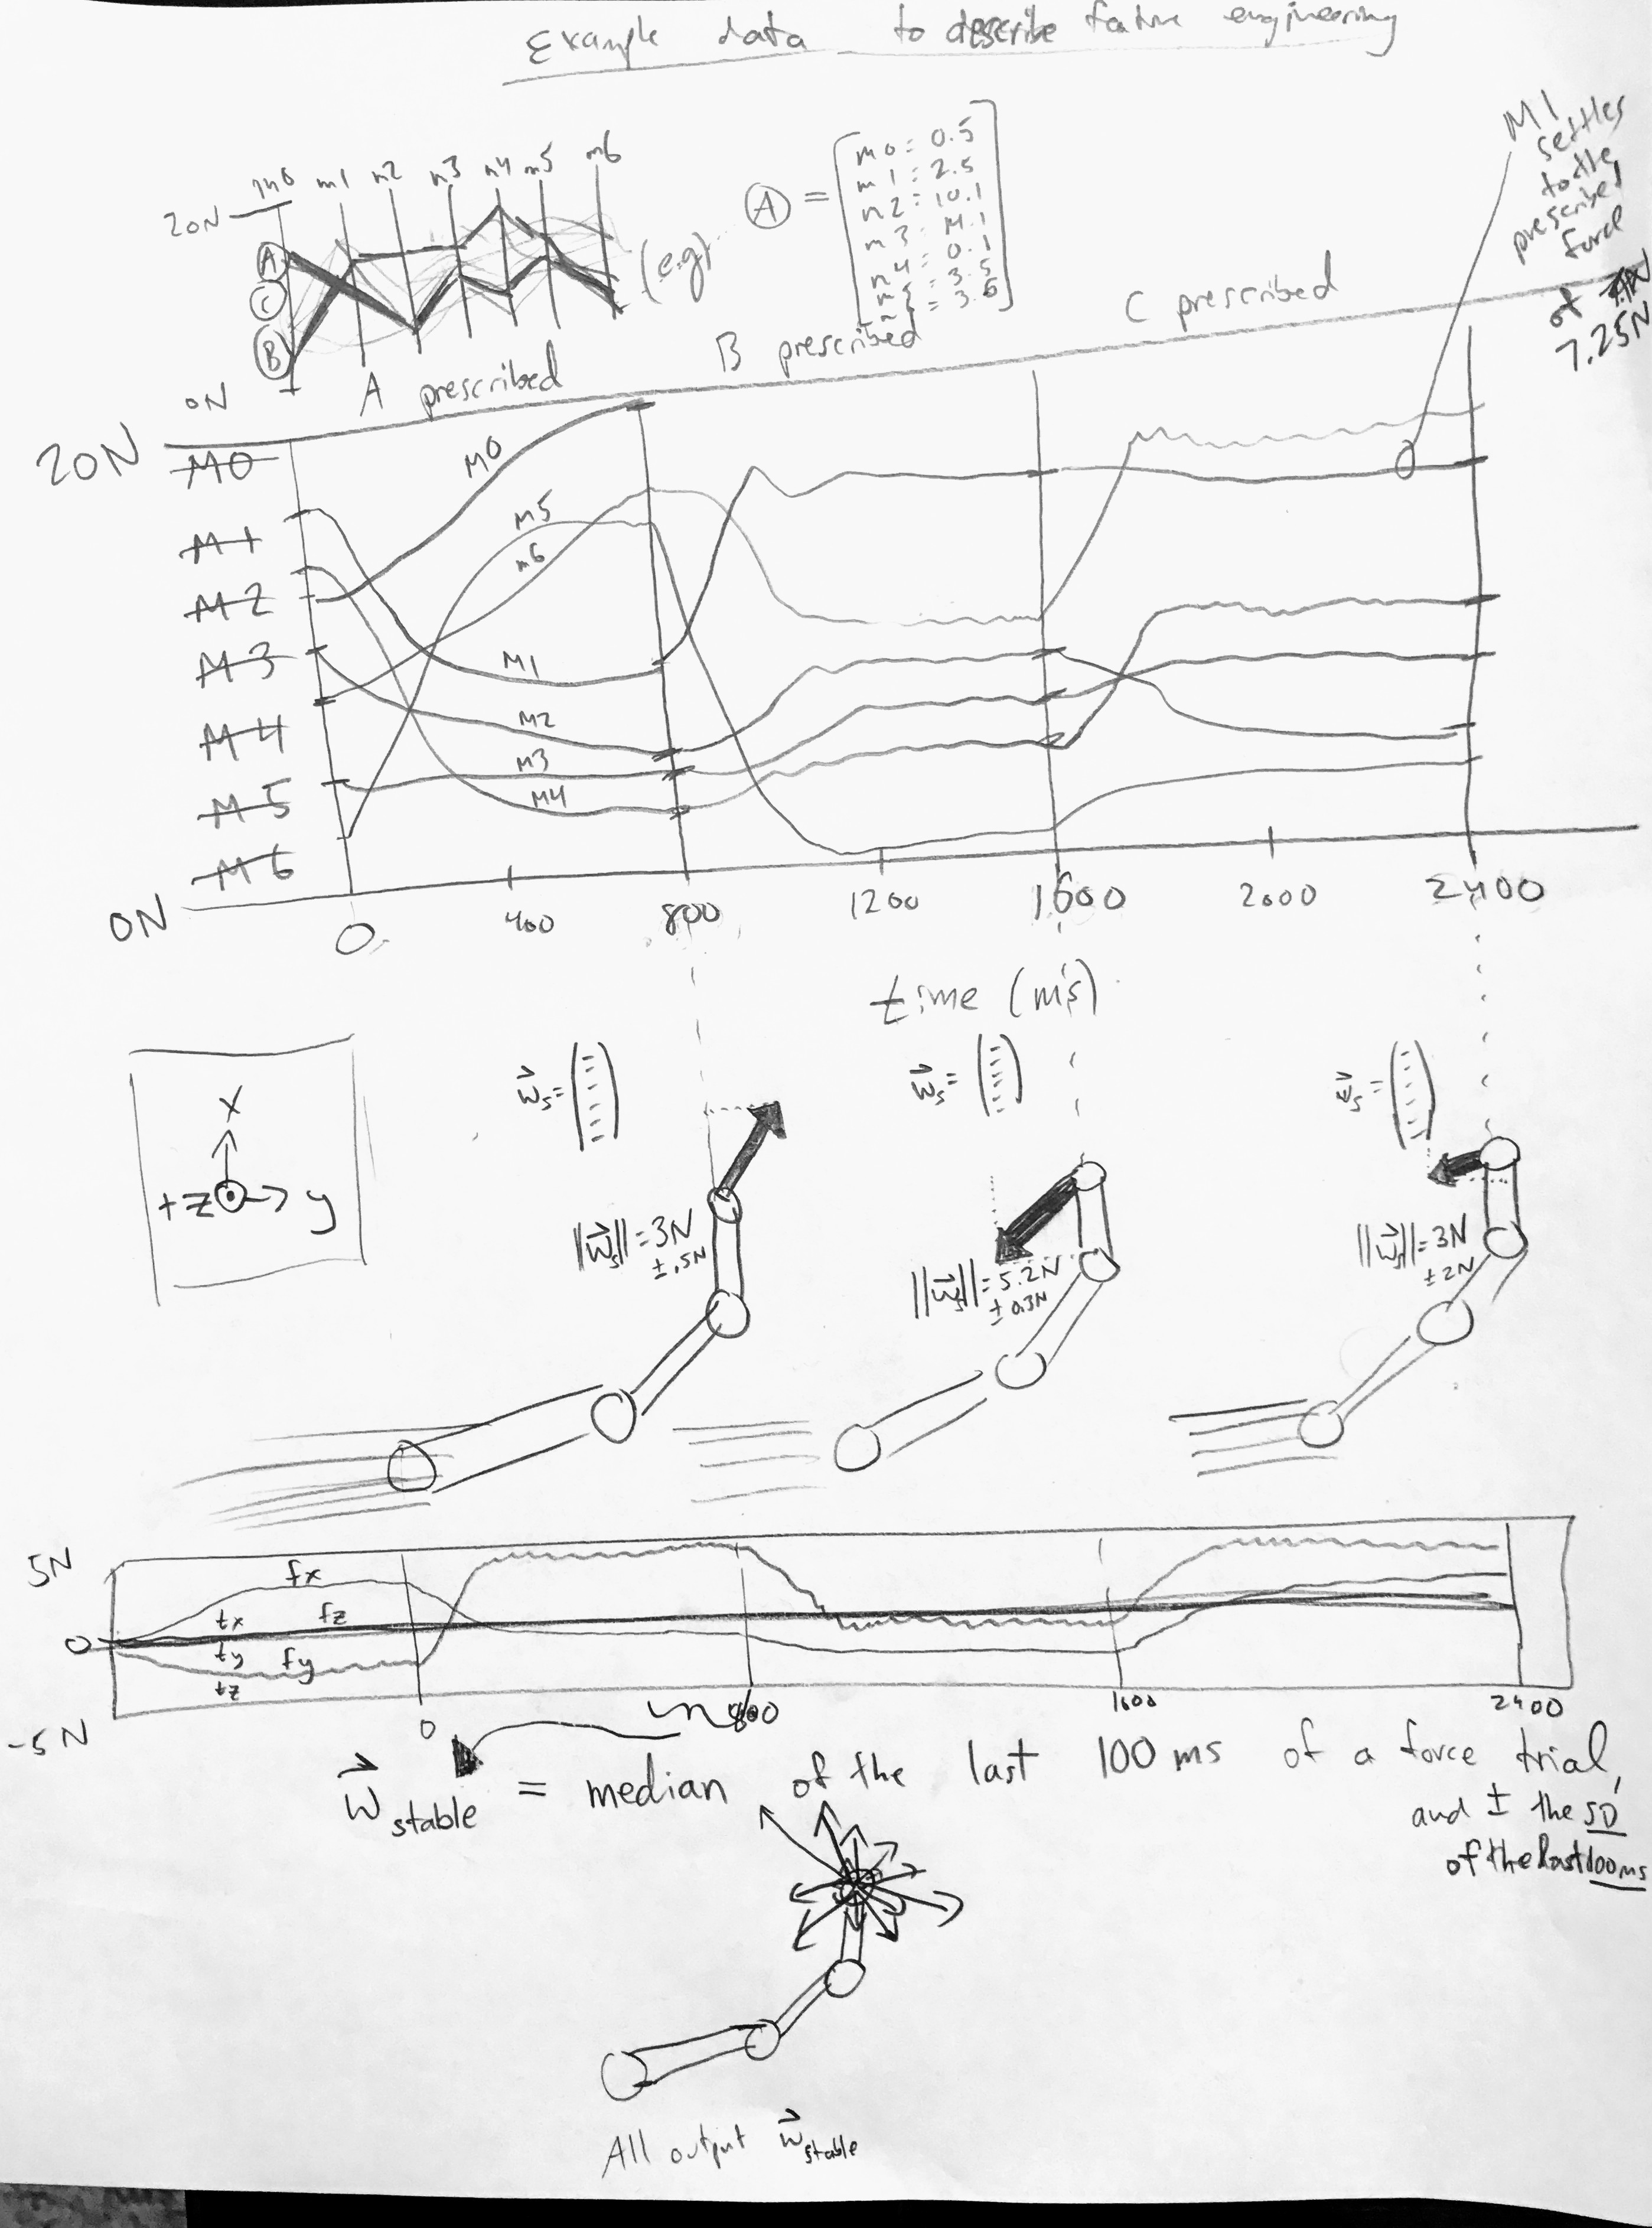
\includegraphics[width=17.5cm]{figures/data_description/data_description.jpg}% This is a *.jpg file
\end{center}
\caption{Description of the data and signals recorded for this analysis. In viewing the SD of measured force once the signal has stablilized (by extracting only the last 100ms) we found the max, first quartile, median, third quartile, and max of SD were X,Y,Z,A,B, respectively.}
\label{fig:data_description}
\end{figure}

\begin{figure}[h!]
\begin{center}
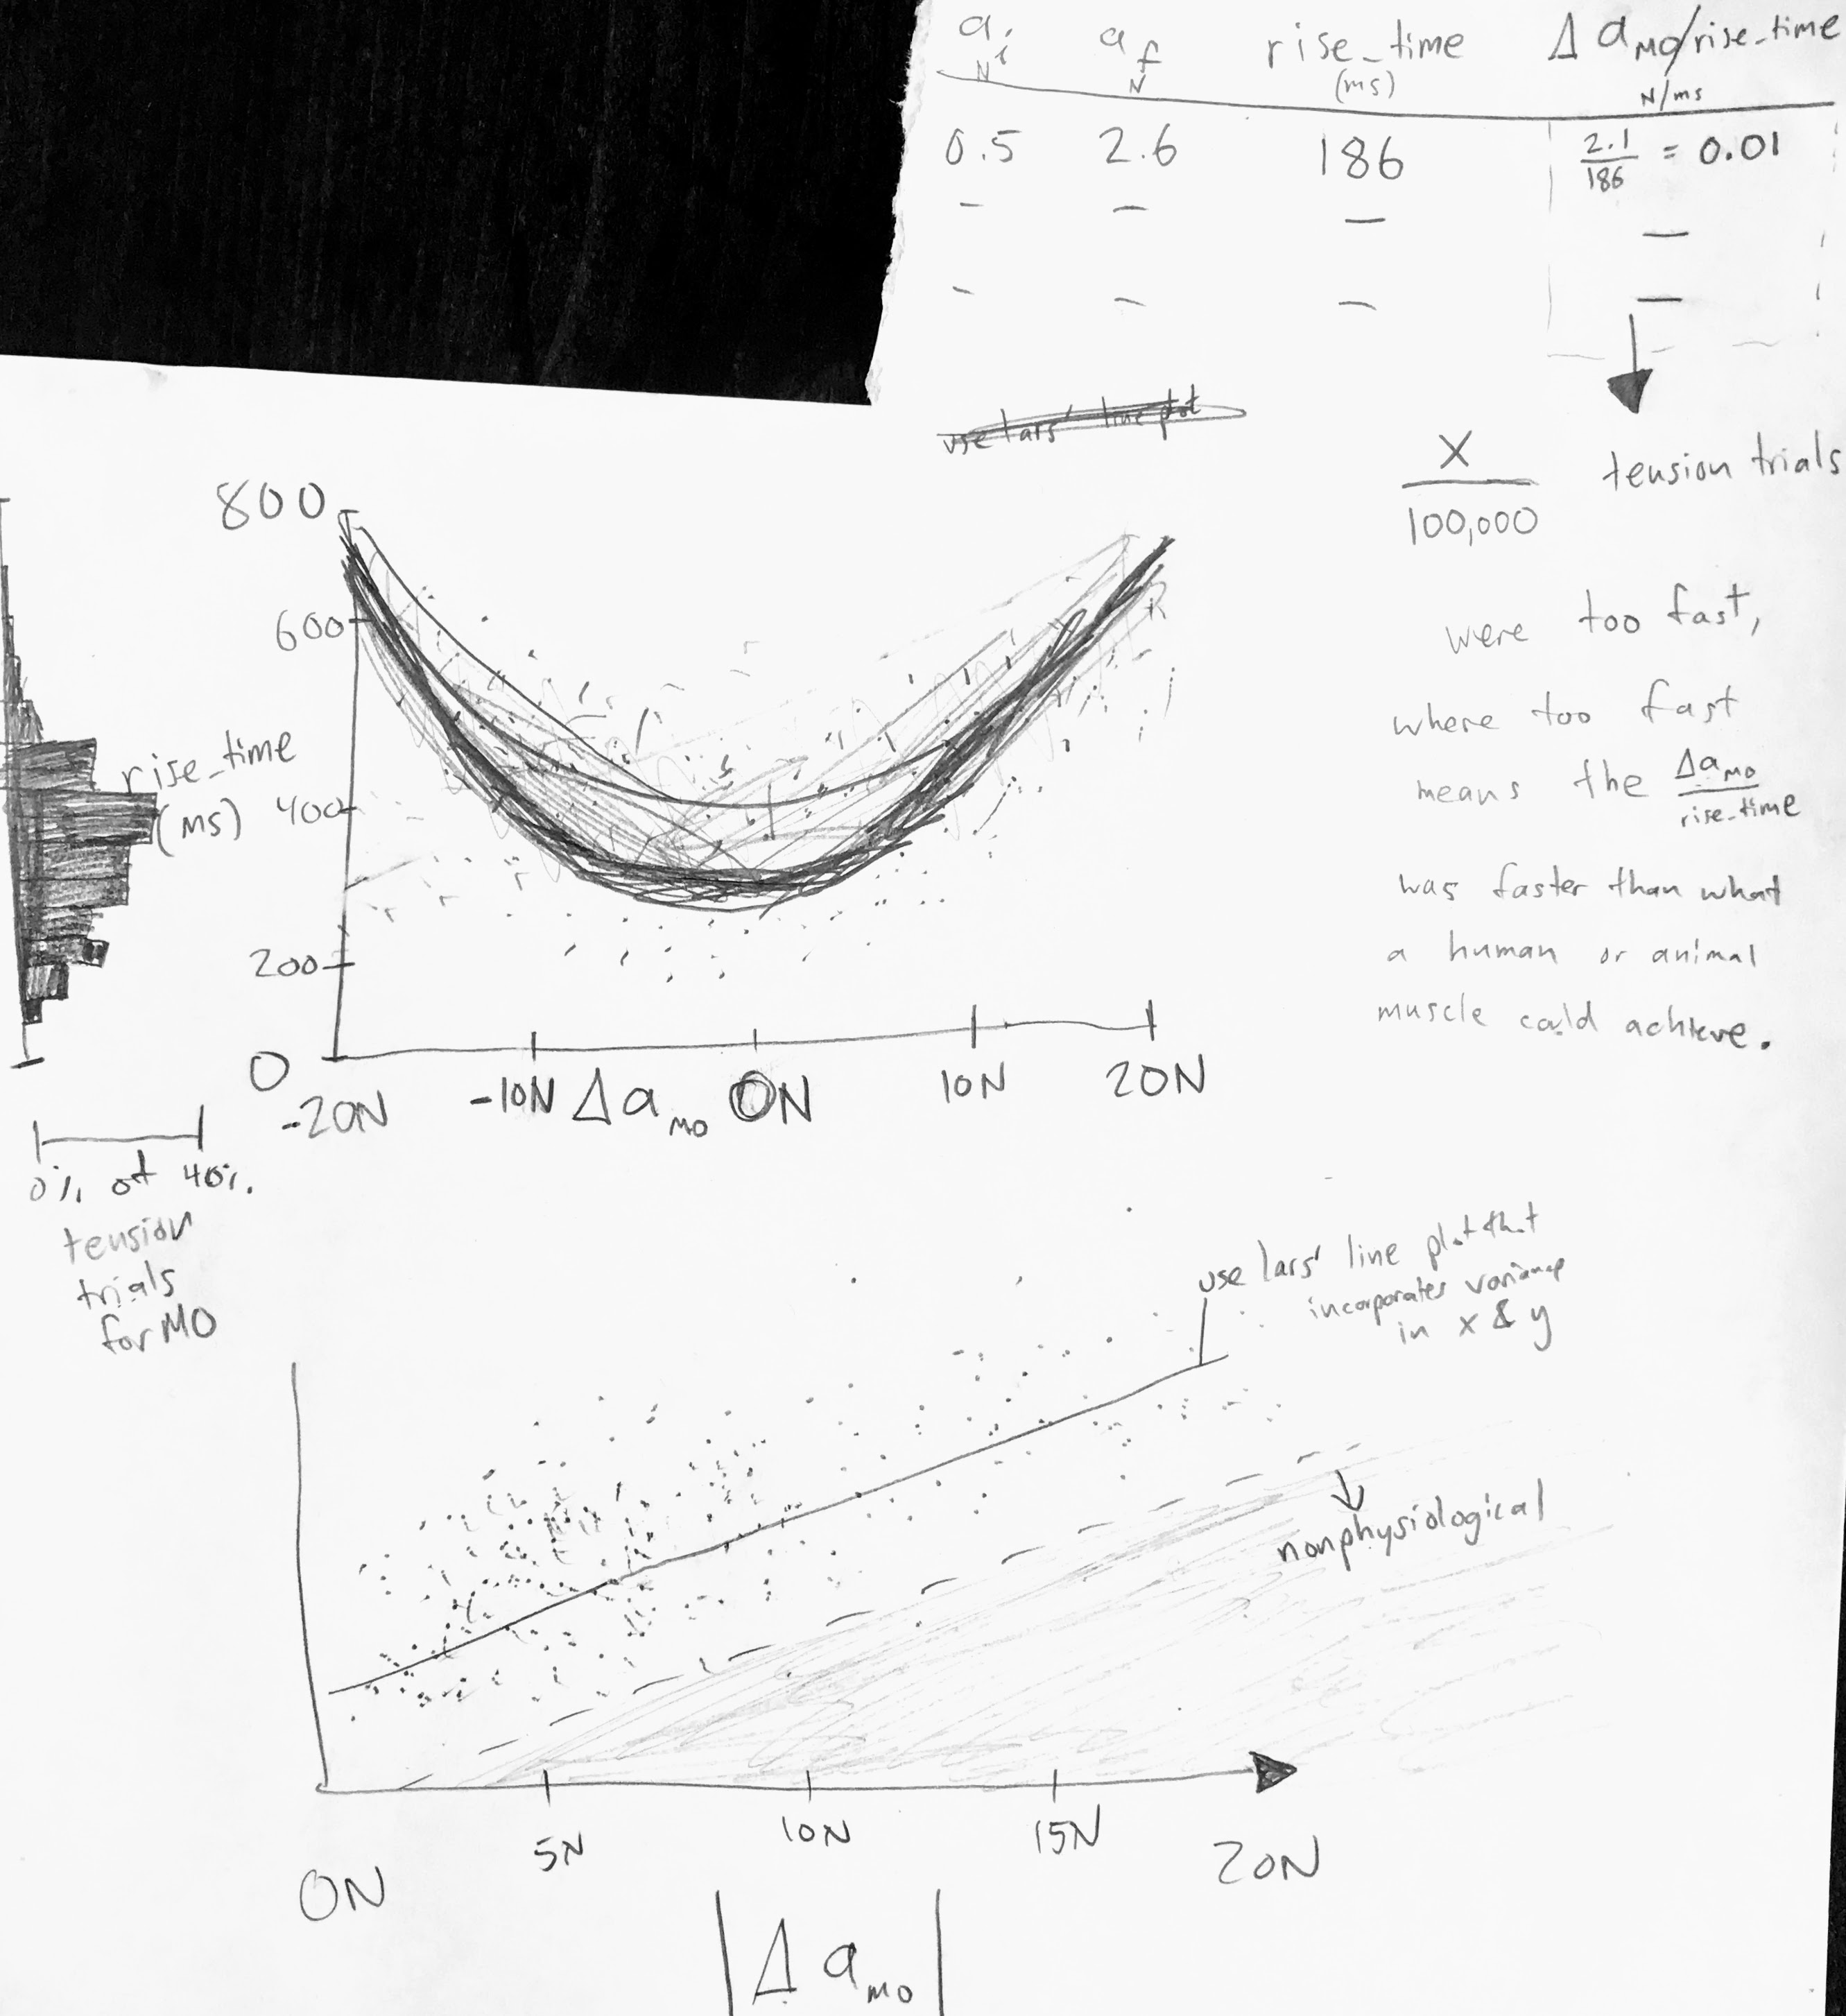
\includegraphics[width=17.5cm]{figures/rise_time_and_delta_activation/rise_time_and_delta_activation.jpg}% This is a *.jpg file
\end{center}
\caption{Rise time and how the change in activation changes the settling time. The input is merely a change in the amplitude of the step. Given a system with the same bandwidth as the model we create for it, you would expect the same settling time. Unless the bandwidth of the dynamic model changes as a function of input amplitude. Otherwise we do not expect that settling time will be different. }
\label{fig:rise_time_and_delta_activation}
\end{figure}

The resultant equation for the linear fit of $t_{rise}$ as a function of $\delta a$ is $t_{rise}$

\begin{figure}[h!]
\begin{center}
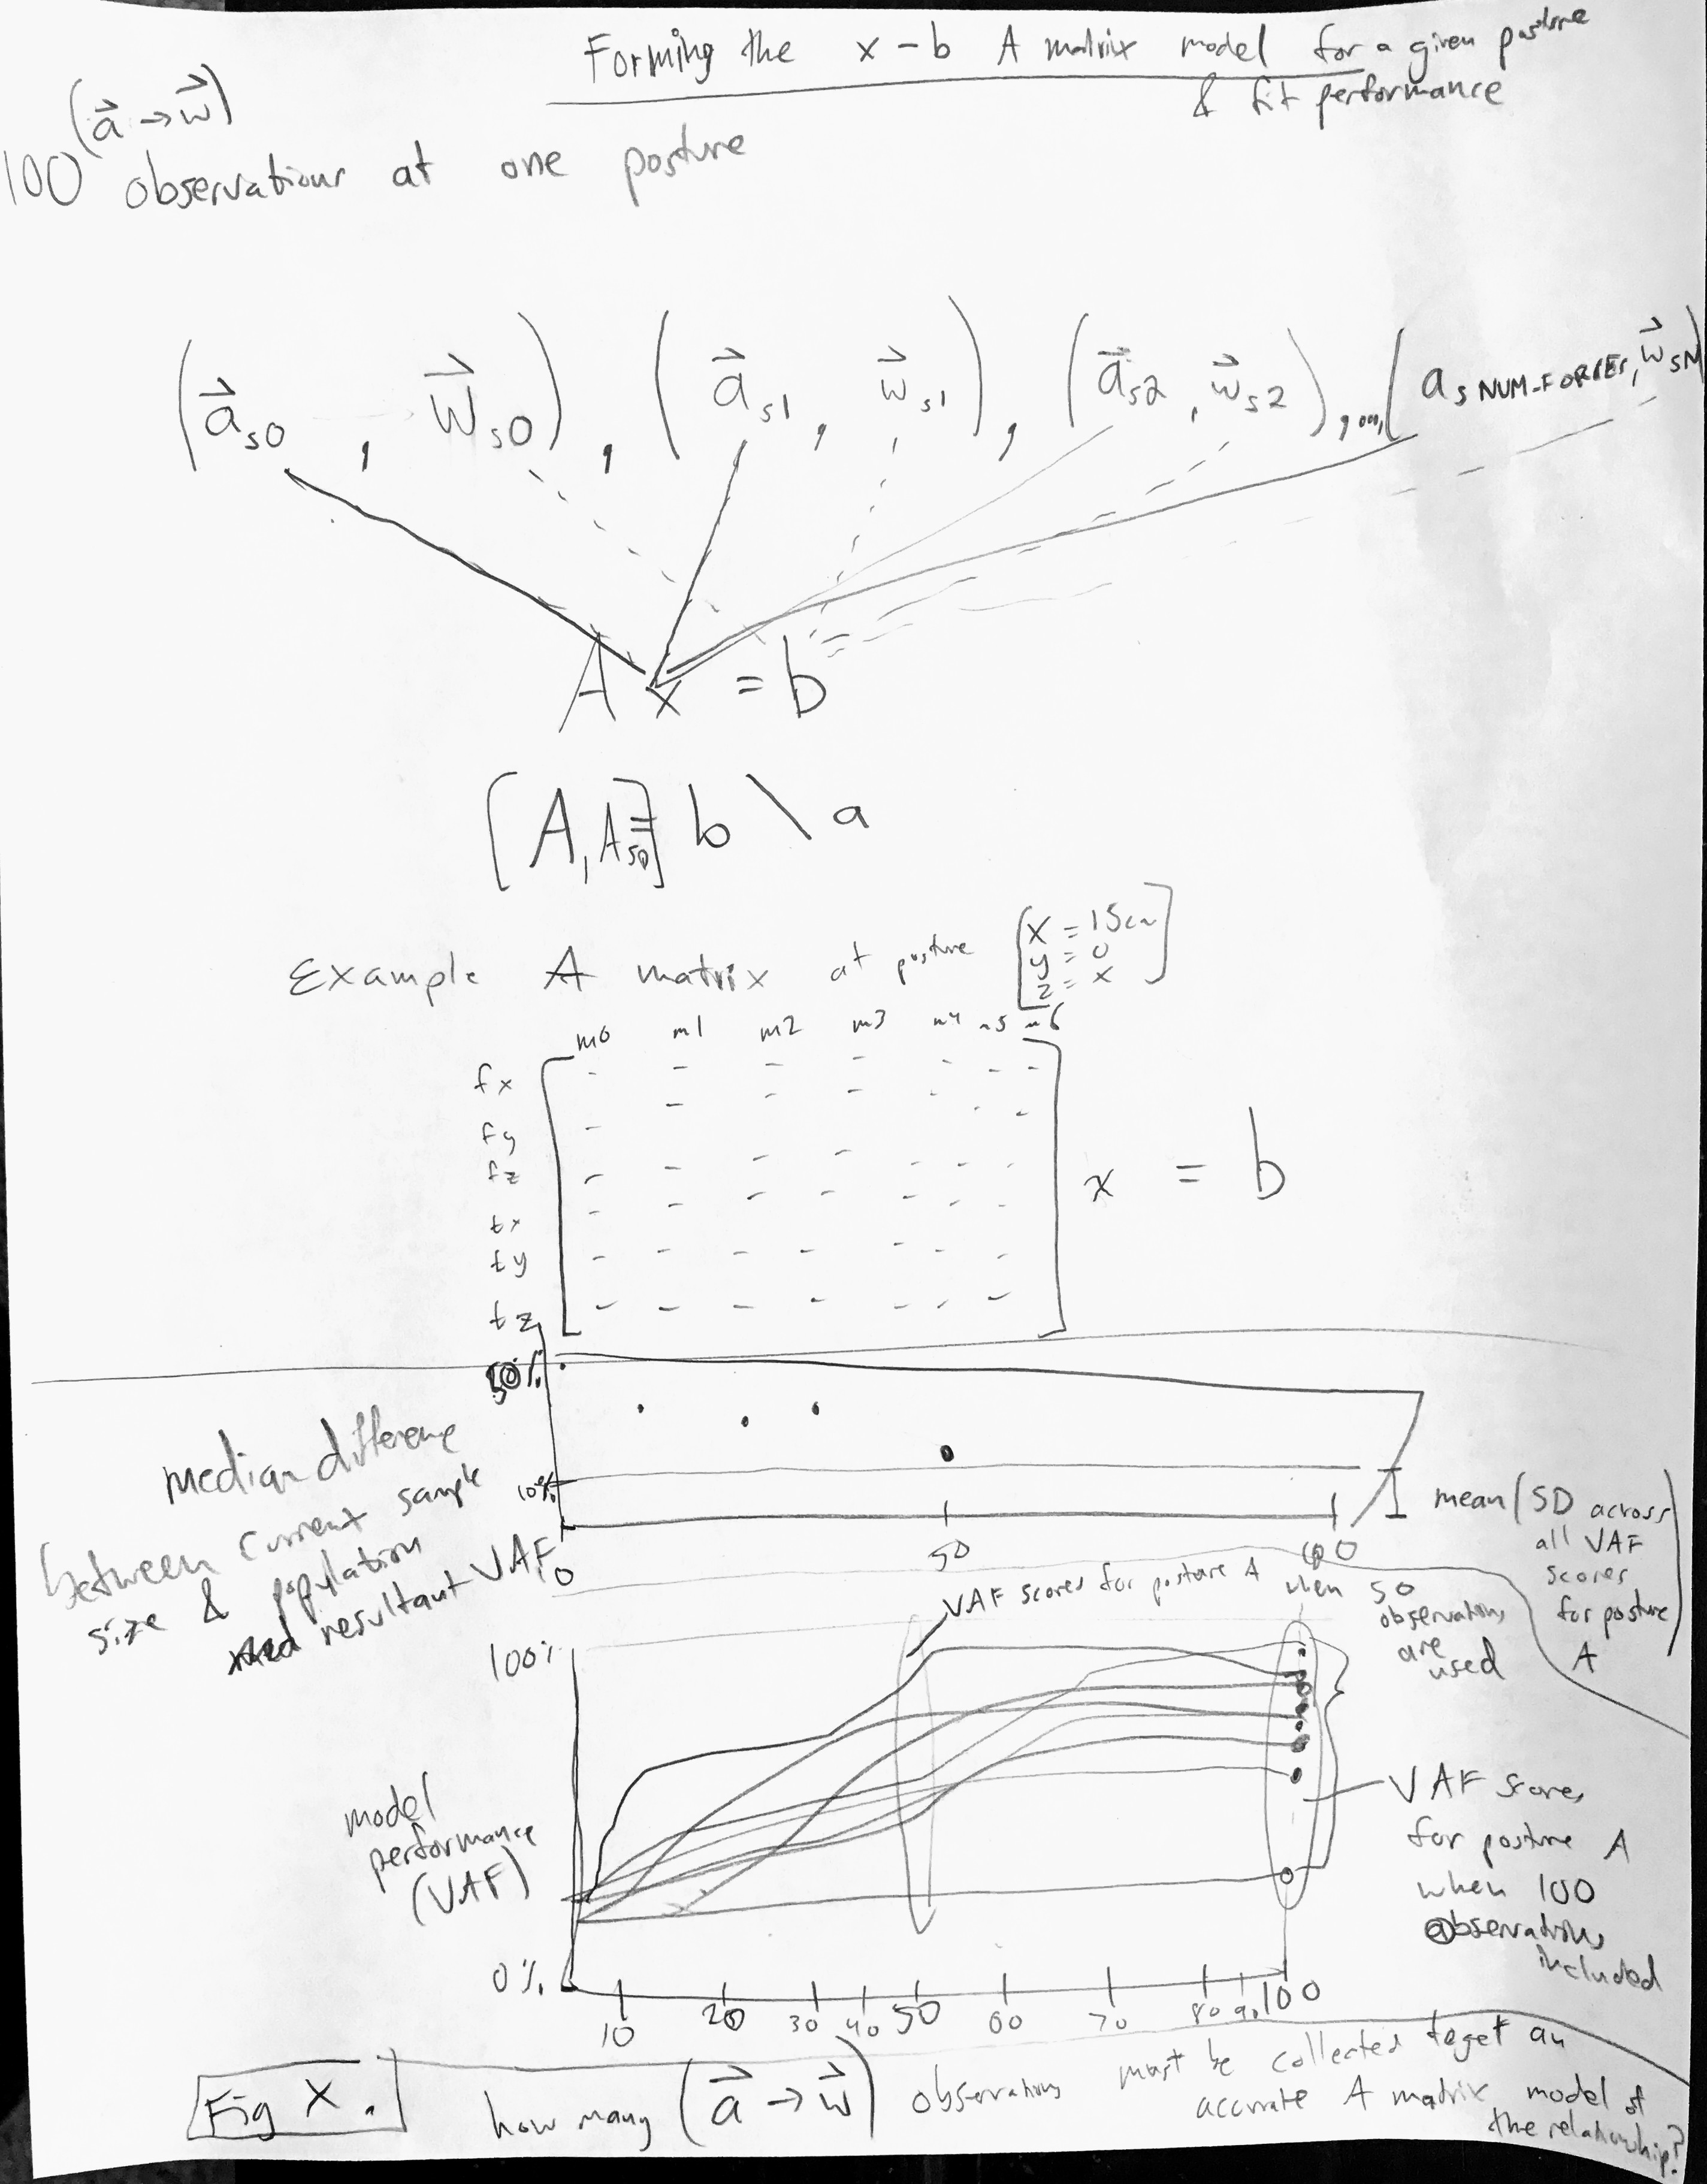
\includegraphics[width=17.5cm]{figures/creating_A_matrix/creating_A_matrix.jpg}% This is a *.jpg file
\end{center}
\caption{Application of linear modeling to tension-to-force relationships }
\label{fig:creating_A_matrix}
\end{figure}

\begin{figure}[h!]
\begin{center}
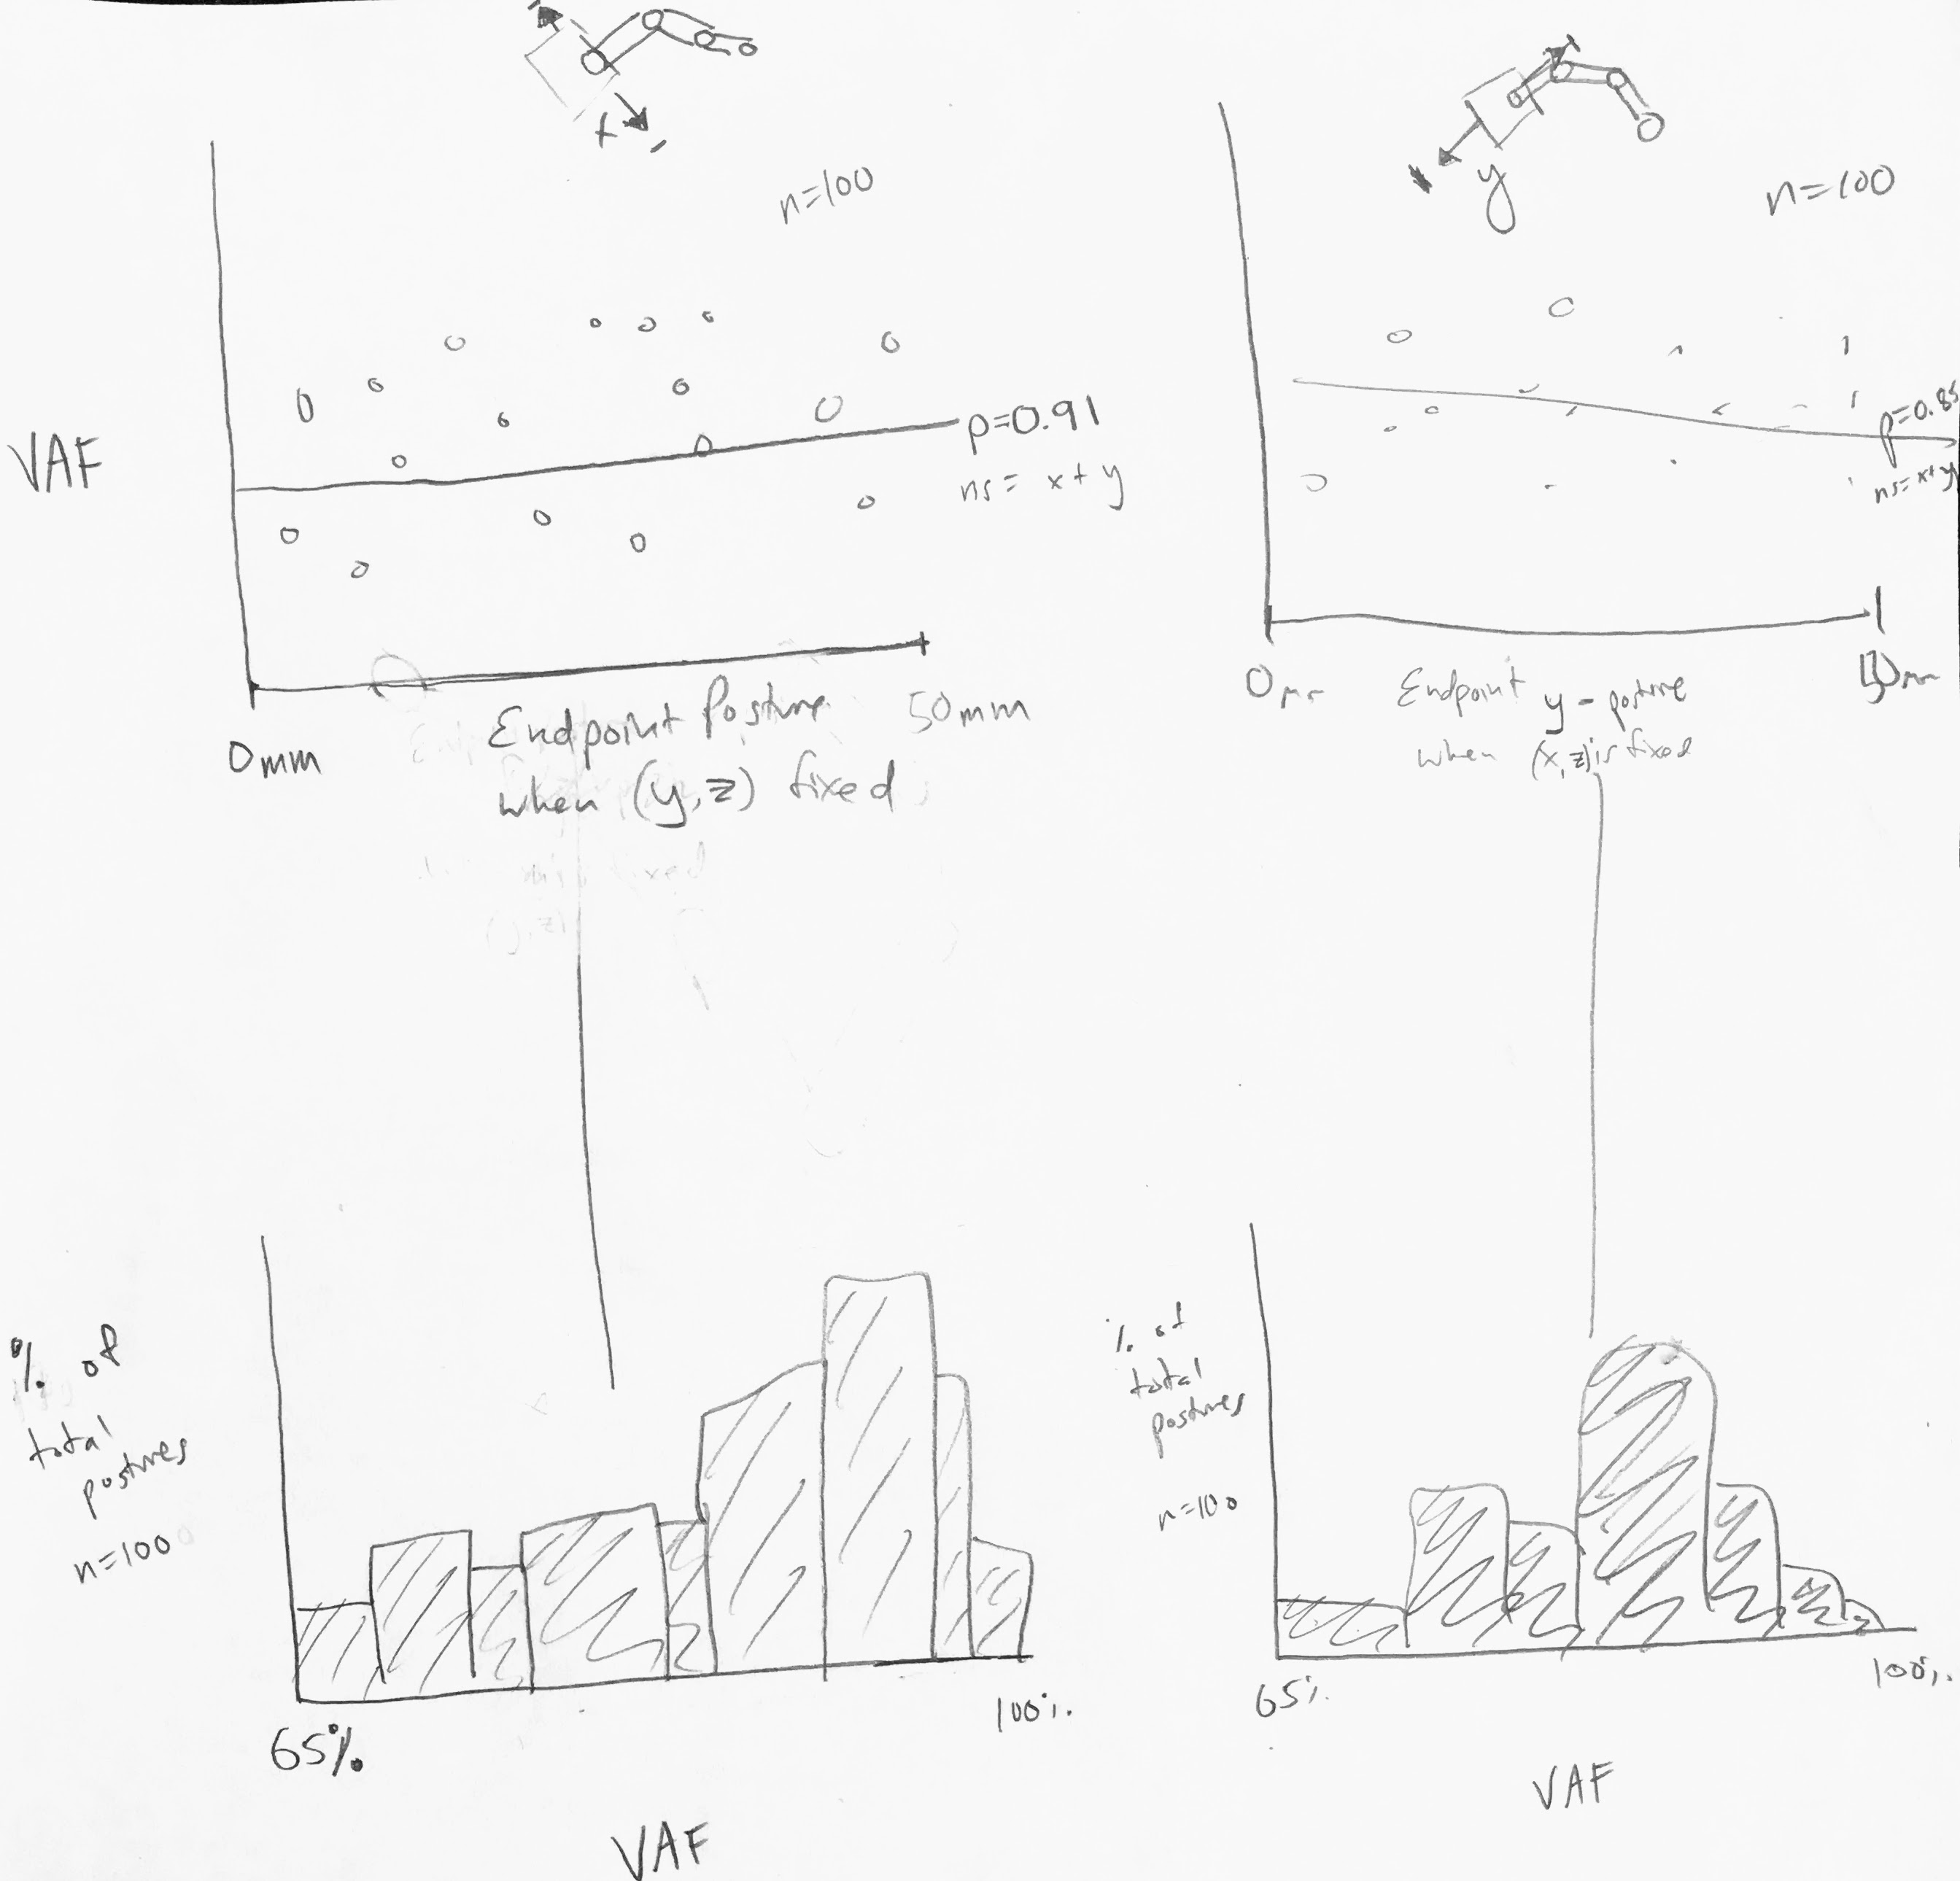
\includegraphics[width=17.5cm]{figures/model_fit/model_fit.jpg}% This is a *.jpg file
\end{center}
\caption{Model fit for a linear matrix in different postures. Fit across the Y posture line (while X and Z were fixed), and the X posture line (while Y and Z were fixed), showed no significant areas of higher or lower model fit (p=0.X, p=0.7, respectively).}
\label{fig:model_fit}
\end{figure}

\begin{figure}[h!]
\begin{center}
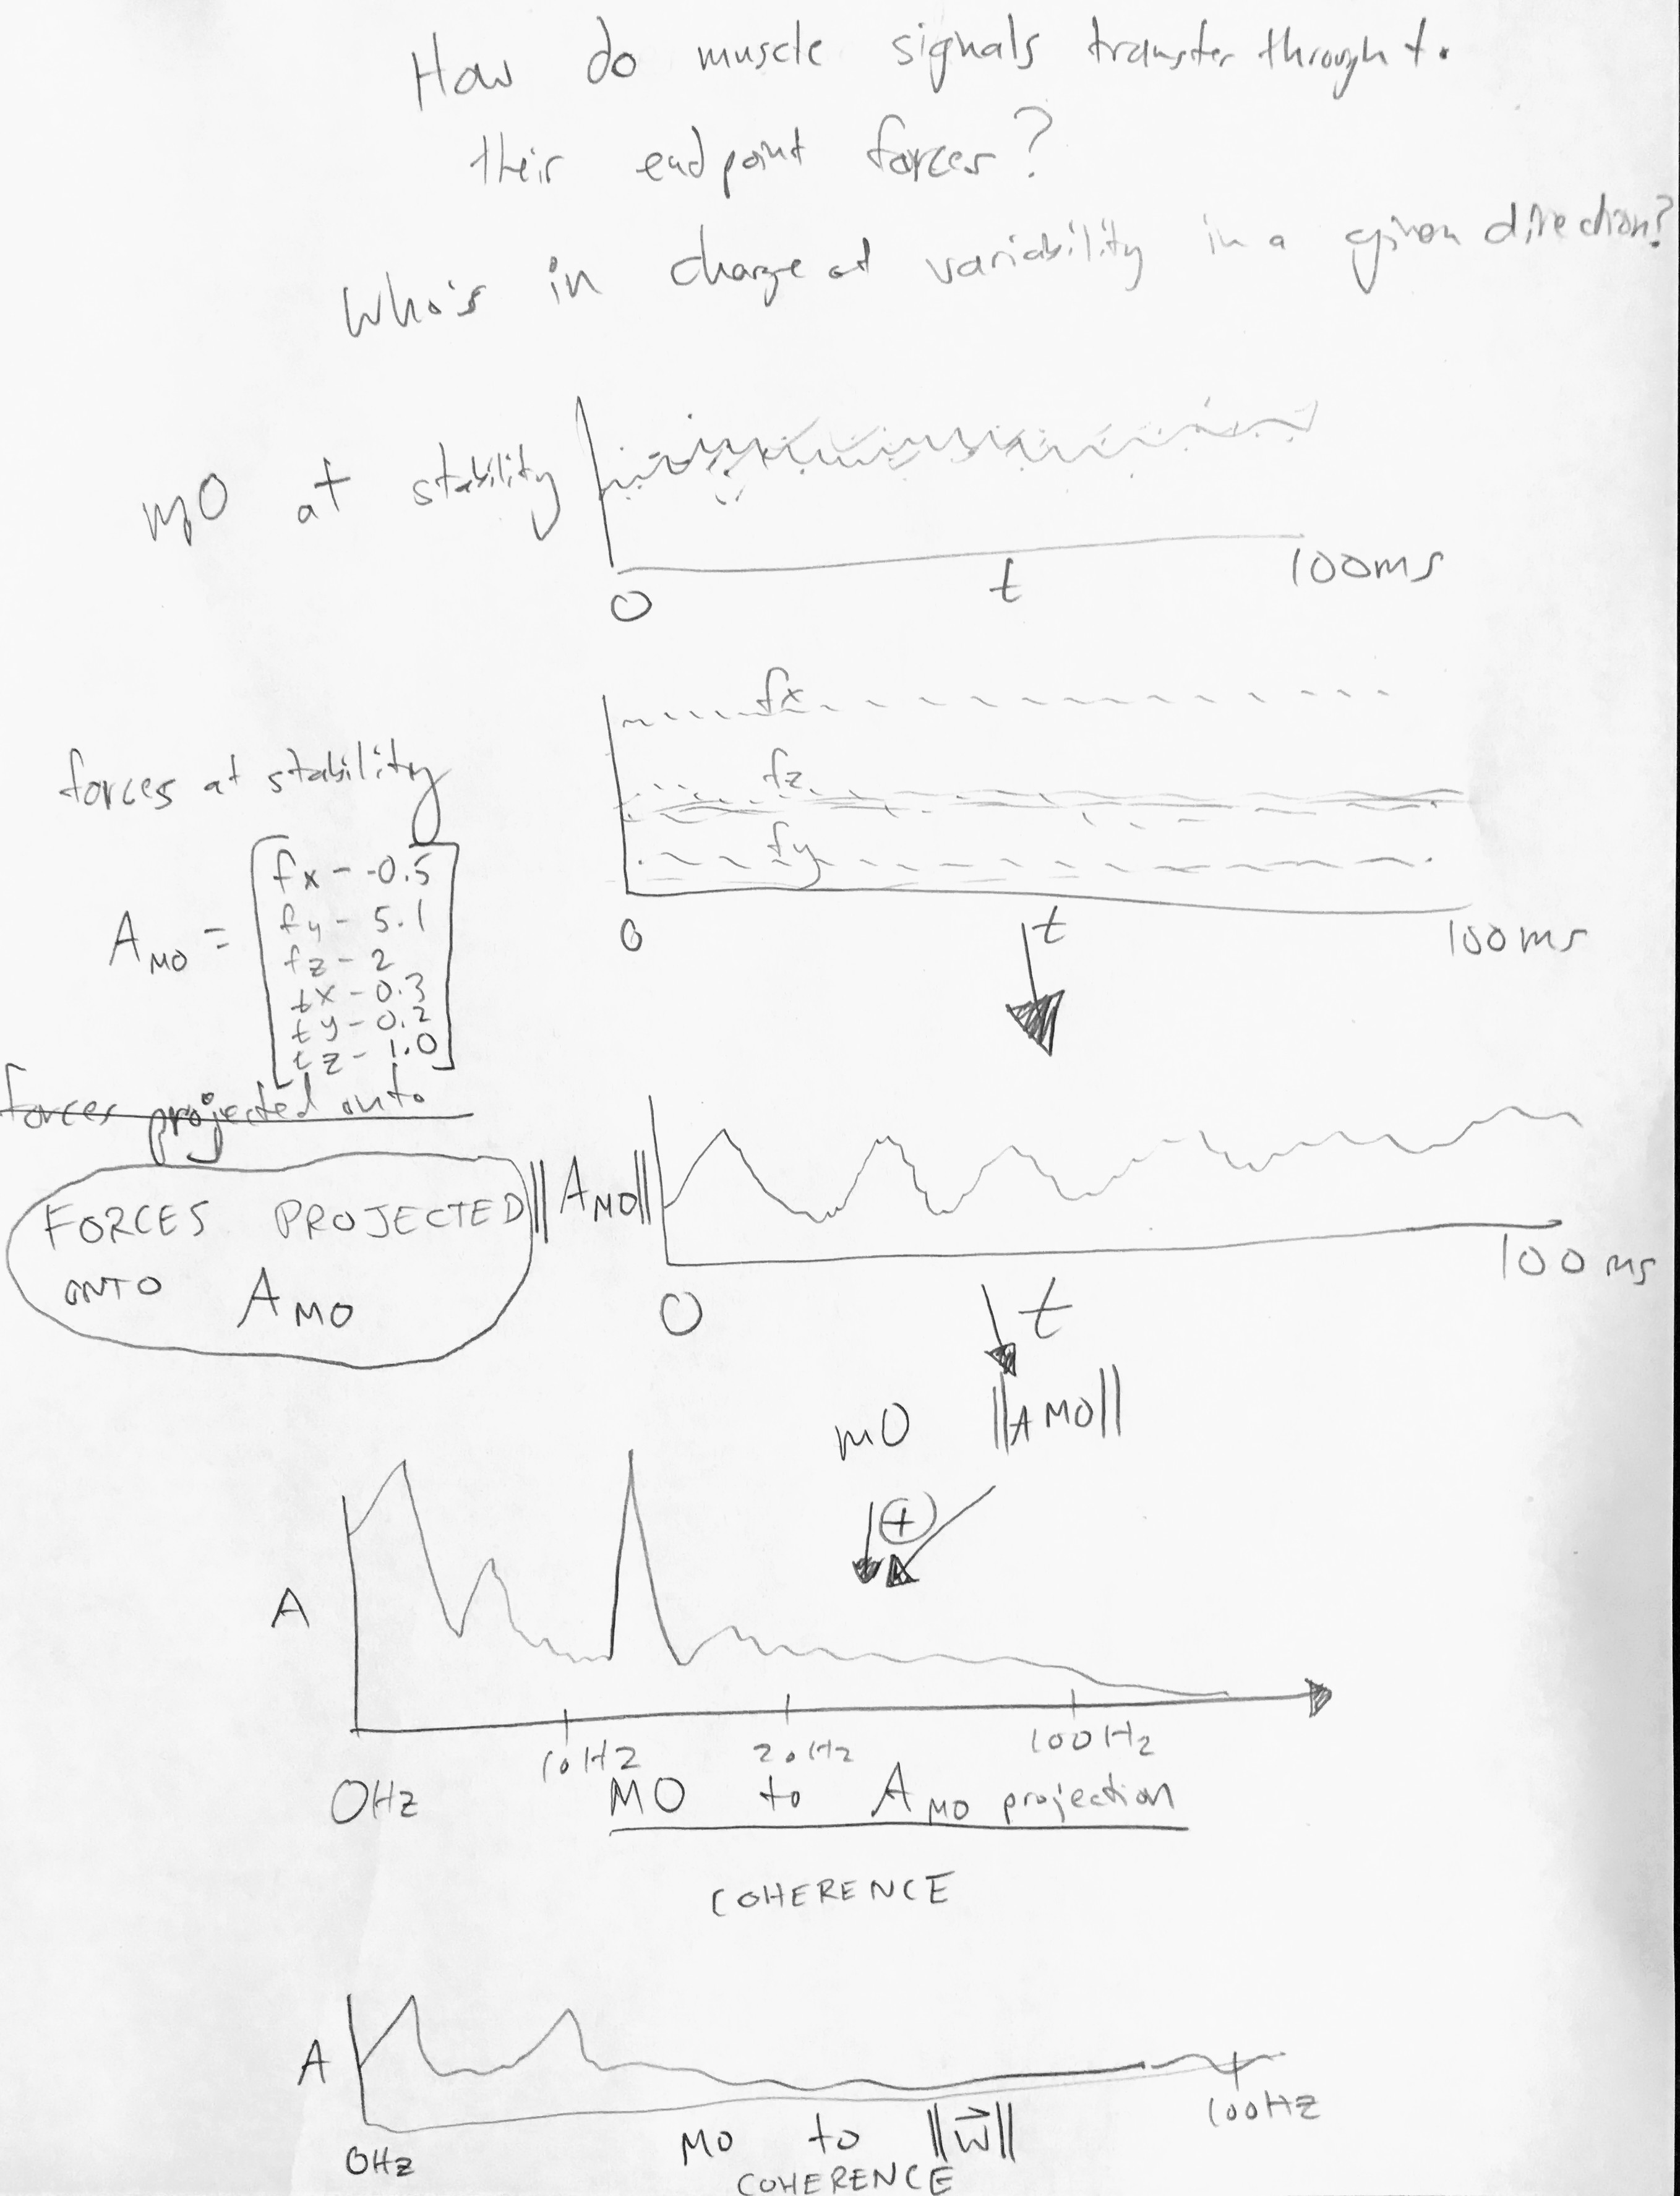
\includegraphics[width=17.5cm]{figures/muscle_force_coherence/muscle_force_coherence.jpg}% This is a *.jpg file
\end{center}
\caption{Tension-to-force coherence across different muscles, and with respect to the linear model's observed tendon contribution}
\label{fig:muscle_force_coherence}
\end{figure}


\begin{figure}[h!]
\begin{center}
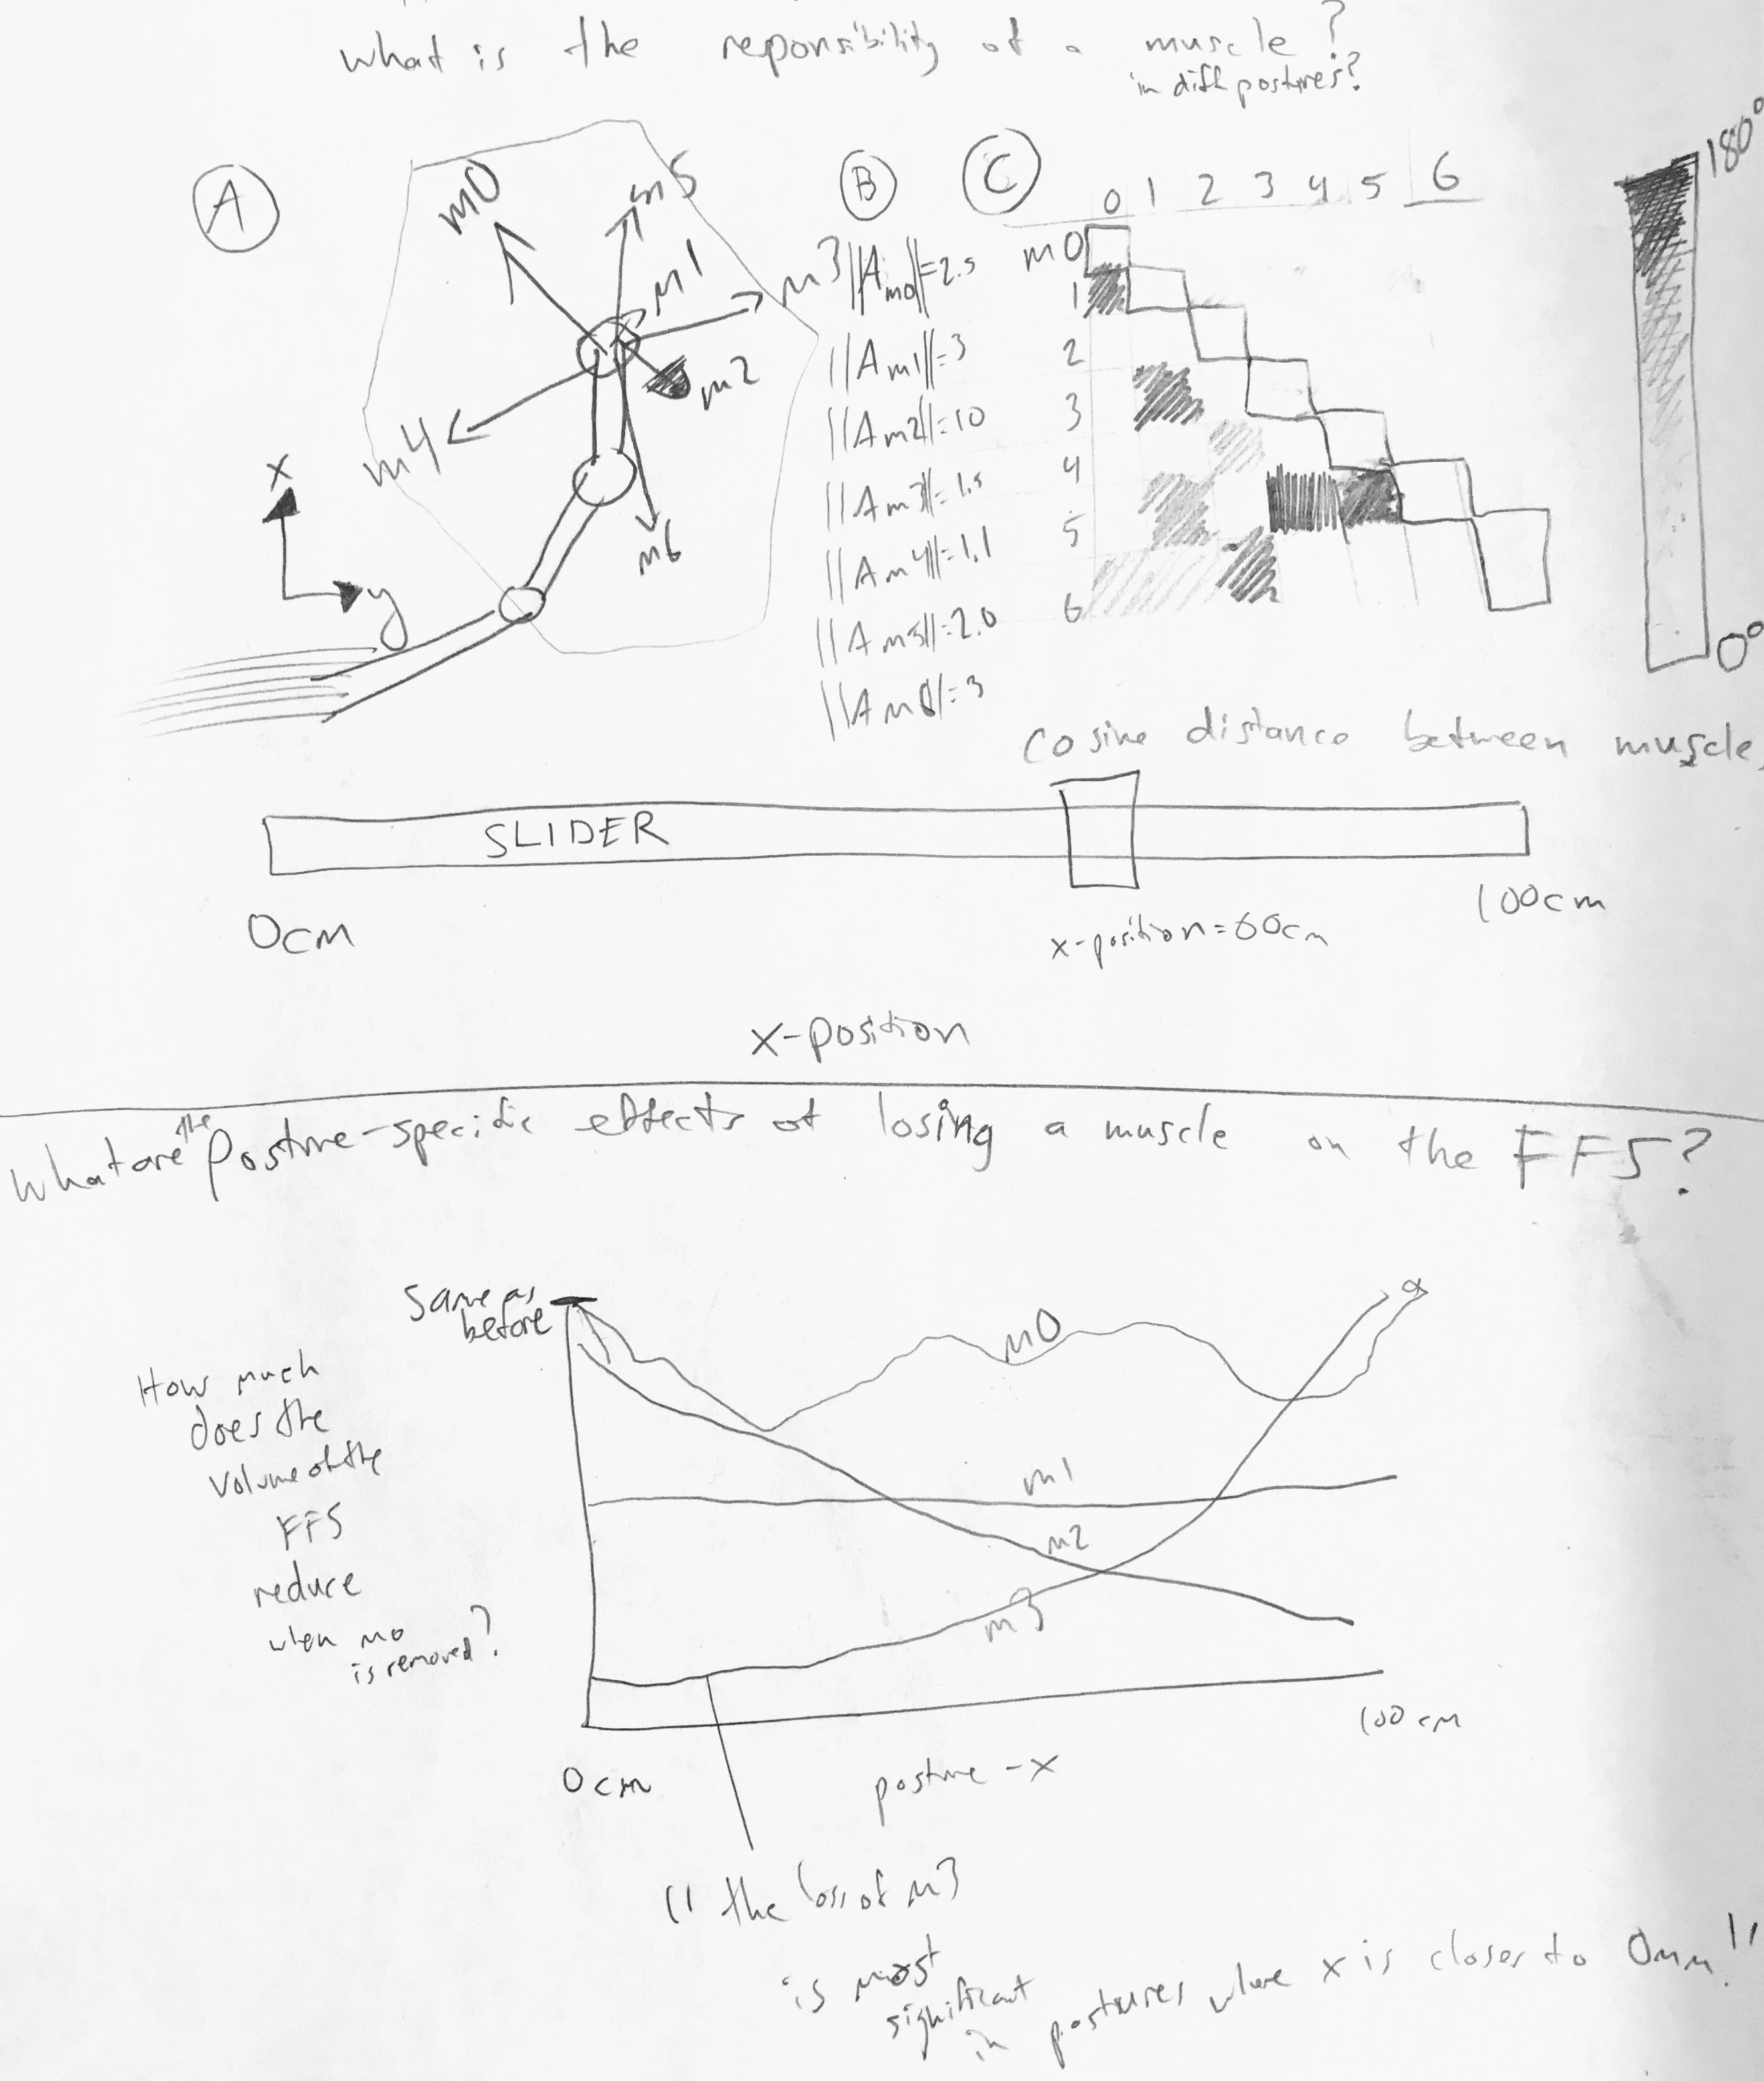
\includegraphics[width=17.5cm]{figures/responsibility_of_a_muscle/responsibility_of_a_muscle.jpg}% This is a *.jpg file
\end{center}
\caption{Responsibility of a muscle in output force space }
\label{fig:responsibility_of_a_muscle}
\end{figure}

\begin{figure}[h!]
\begin{center}
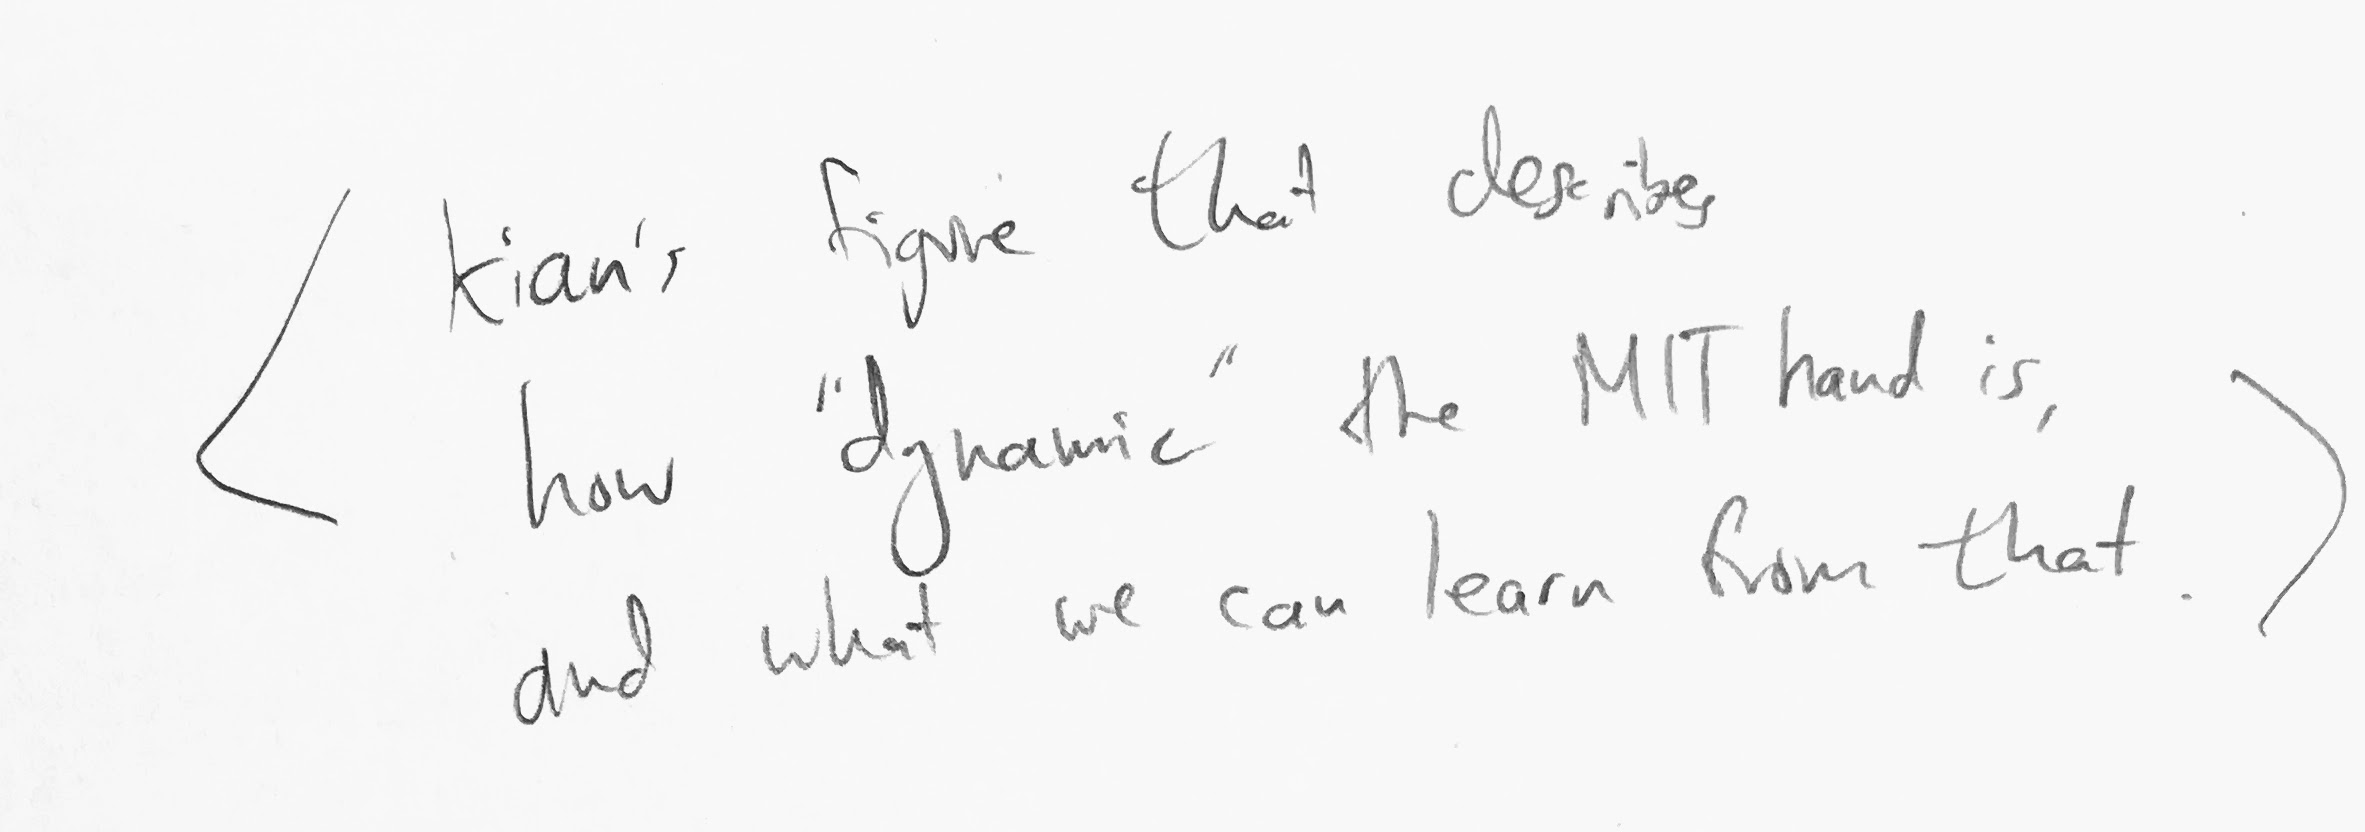
\includegraphics[width=17.5cm]{figures/dynamics_vs_statics/dynamics_vs_statics.jpg}% This is a *.jpg file
\end{center}
\caption{KIAN TODO}
\label{fig:dynamics_vs_statics}
\end{figure}


%%% If you don't add the figures in the LaTeX files, please upload them when submitting the article.
%%% Frontiers will add the figures at the end of the provisional pdf automatically
%%% The use of LaTeX coding to draw Diagrams/Figures/Structures should be avoided. They should be external callouts including graphics.

\end{document}
